The experiments of Section~\ref{sec:experiments} involve several numerical algorithms for solving traffic assignment problems. These all follow the fixed-point iteration depicted in Figure \ref{fig:iteartion} between the model $F$ and the update function of the numerical method, $U$. $U$ is allowed to have a state. 
%In the figure, the top block represents the traffic model $F$, which maps candidate demand assignments $h^k$ into path costs $c^k$. The bottom block is a solver update function $U$, which updates the candidate assignment based on information from previous iterations. The index $k$ is incremented in each iteration, and the process continues until convergence is reached.
The numerical algorithms use the
\textit{all-or-nothing assignment at iteration $k$},  $y^k$:
%by placing all of the demand for each OD pair $w$ onto paths whose entry in $c^k$ is minimum amongst paths in $\mathcal{P}_w$. To express this mathematically, we introduce the notation $c^k_p$ for the cost on path $p$ at iteration $k$, $c^k_w=\{c^k_p\}_{p\in\mathcal{P}_w}$, and $y^k_p$ for the demand on path $p$ in the all-or-nothing assignment. Then,
\begin{equation}
\label{eq:allornothing}
y^k_p = \left\{
\begin{tabular}{ll}
$d_w/s$ & $p\in\underset{p'\in\mathcal{P}_w}{\text{argmin }} c^k_{p'} $ \\
0 & otherwise
\end{tabular}
\right.
\end{equation}
Here $s=|\underset{p\in\mathcal{P}_w}{\text{argmin }} c^k_{p}|$. The superscript $k$ is the iteration index of the numerical solver.
The all-or-nothing assignment is also used in the  termination criterion ($\epsilon>0$):
\begin{equation}
\label{termination_criterion}
\text{Stop if }
{\frac {\langle c^k,y^k-h^k \rangle} {\langle y^k, c^k\rangle}} \leq \epsilon
\end{equation}
% Here $\epsilon$ is a small positive number. 

\begin{figure}[h]
    \centering
    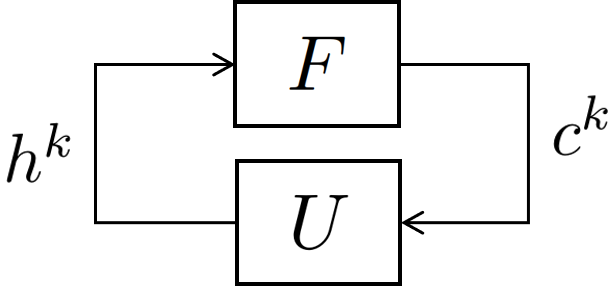
\includegraphics[width=0.4\linewidth]{figs/iteration.png}
    \caption{Generic iteration}
    \label{fig:iteartion}
\end{figure}

\subsection{Frank-Wolfe Algorithm (FW)}
FW 
\cite{fukushima1984modified} 
is a well-known method for solving convex optimization problems which is especially well suited for network problems. The algorithm was used in \cite{thai2016negative} to solve large-scale static traffic assignment problems. The update function of FW is,
\begin{equation}
h^{k+1} = h^k +\alpha\; (y^k - h^k)
\end{equation}
with $\alpha$ set such that $h^{k+1}$ minimized the cost function over the chord between 
$y^k$ and $h^k$.

% the following steps:
% \begin{enumerate}
% \item Compute $y^k$ with Eq. (\ref{eq:allornothing}).
% \item Calculate $d^k = $
% \item Calculate the step size $\alpha$ as the solution to the following line-search problem:
% \begin{equation}
% \begin{aligned}
% & \underset{\alpha}{\text{minimize}}
% & & \langle F(h^k + \alpha\; d^k), d^k \rangle \\
% & \text{subject to}
% & & \alpha \in [0,1]
% \end{aligned}
% \end{equation}
% \item $$.
% \end{enumerate}

% Terminate if Eq. (\ref{termination_criterion}) is met.

\subsection{Method of Successive Averages}
The Method of Successive Averages (MSA) is a heuristic that does not guarantee convergence to a solution, but has generally been found to work well \cite{nie2010solving}. The algorithm advances with,
\begin{equation}
h^{k+1} = (1-1/k)h^k + (1/k) y^k
\end{equation}

% \begin{enumerate}
% \item Compute $y^k$ with Eq. (\ref{eq:allornothing}).
% \item With step size $\alpha = 1/k$,  . 
% \end{enumerate}
% Terminate if Eq. (\ref{termination_criterion}) is met.

\subsection{Extra Projection Method}
The Extra Projection Method (EPM) is based on the Euclidean projection operator, defined as,
\begin{equation}
\Pi_\mathcal{H}(x) = \underset{h}{\text{argmin}}\{\lVert h-x\rVert_2 \; : \;h \in\mathcal{H} \}
\end{equation}
%where $\lVert\cdot\rVert$ is the Euclidean norm. 
The EPM guarantees convergence when $F$ is Lipschitz continuous and pseudo-monotone \cite{nie2010solving}. 
%Use $L$ to denote the Lipschitz constant of $F$. 
$\tau^k$ is a number that is smaller than the Lipschitz constant of $F$. The update function of EPM is,
\begin{equation}
h^{k+1} = \Pi_\mathcal{H}(h^k - \tau^k F(z^k))
\end{equation}
where $z^k = \Pi_\mathcal{H}(h^k - \tau^k c^k)$. If the Lipschitz constant of $F$ is unknown, then \cite{nie2010solving} proposes the following update equation for $\tau^k$:
\begin{equation}
\tau^{k+1} = \left\{
\begin{tabular}{ll}
$\sigma\;\tau^k$ & 
if $y^{k+1}-y^k < 0$ and $\frac{|y^{k+1}-y^k|}{|y^k|}> \mu$ \\
$\tau^k$ & otherwise
\end{tabular}
\right.
\end{equation}
%Here $y^{k+1}$ and $y^k$ are the all-or-nothing assignments corresponding to $h^k$ and $h^{k+1}$ respectively. 
$\mu$ and $\sigma$ are scalars between 0 and 1.
